\documentclass[usenames, dvipsnames]{beamer}
\usetheme{metropolis}           % Use metropolis theme
%\usecolortheme{seahorse}
\usepackage[utf8]{inputenc}
\usepackage{graphicx}
\usepackage{xcolor}
\usepackage[normalem]{ulem}
\usepackage{varwidth}
\usepackage{listings}
\DeclareRobustCommand{\hsout}[1]{\texorpdfstring{\sout{#1}}{#1}}
\newcommand\teacher[1]{\begin{flushright}\small\textit{#1}\end{flushright}}

\title{Blockchain: Pizza til \hsout{\$21.000.000} \$26.000.000}
\date{13. Oktober, 2017}
\author{mathias@fleig.io}
\institute{Datalogisk Institut \\ Københavns Universitet}
\begin{document}
  \maketitle
  \section{Motivation}
  \begin{frame}{Motivation}
    \center Hvad vil det sige at \textcolor{BurntOrange}{eje} en bitcoin?
  \end{frame}
  \begin{frame}{Motivation}
      \center \textcolor{BlueViolet}{Digital signatures}, \textcolor{Magenta}{Proof of work}, \center \textcolor{SpringGreen}{Cryptographic hash functions}, \textcolor{Emerald}{Assymetric Cryptopgraphy}...
  \end{frame}
  \begin{frame}{Motivation}
    \center Hvorfor er Blockchain så \textcolor{SeaGreen}{komplekst}?
  \end{frame}
  \begin{frame}{Motivation}
      \center "For every complex problem there is an answer that is clear,
			   simple, and \textcolor{red}{wrong}." \textemdash \ H. L. Mencken
  \end{frame}

  \begin{frame}{Motivation}
    \begin{figure}[ht!]
    \centering
    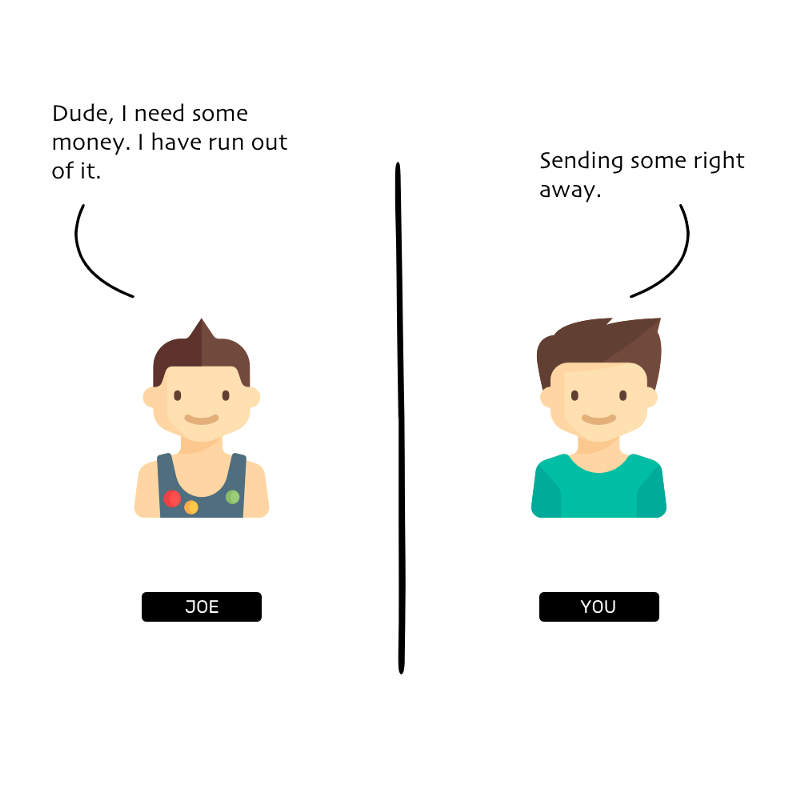
\includegraphics[width=80mm]{images/send_with_bank1.png}
    \end{figure}
  \end{frame}
  \begin{frame}{Motivation}
    \begin{figure}[ht!]
    \centering
        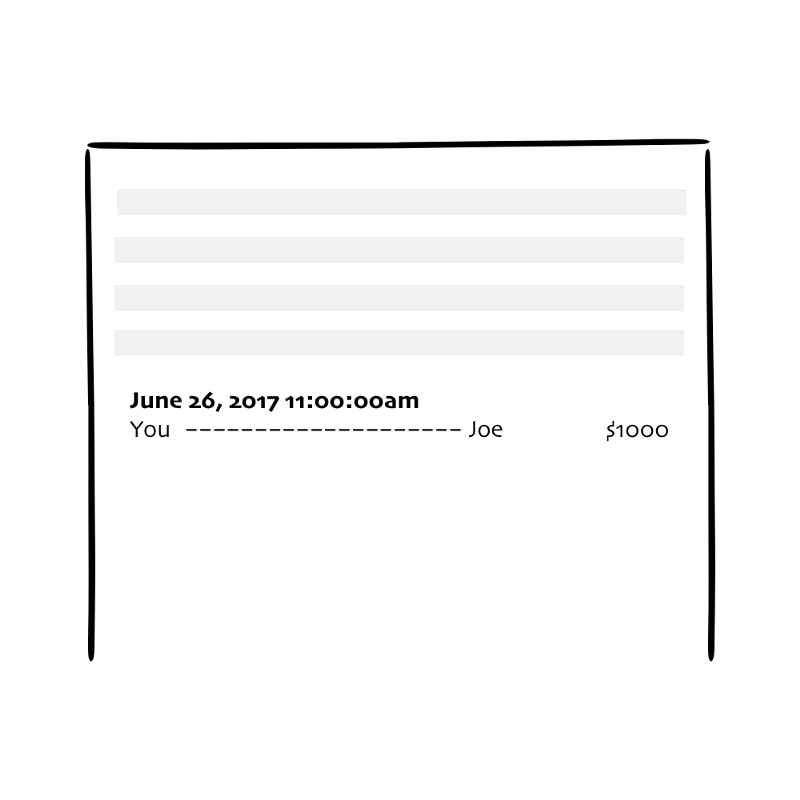
\includegraphics[width=80mm]{images/send_with_bank2.png}
    \end{figure}
  \end{frame}
  \begin{frame}{Motivation}
    \begin{figure}[ht!]
    \centering
    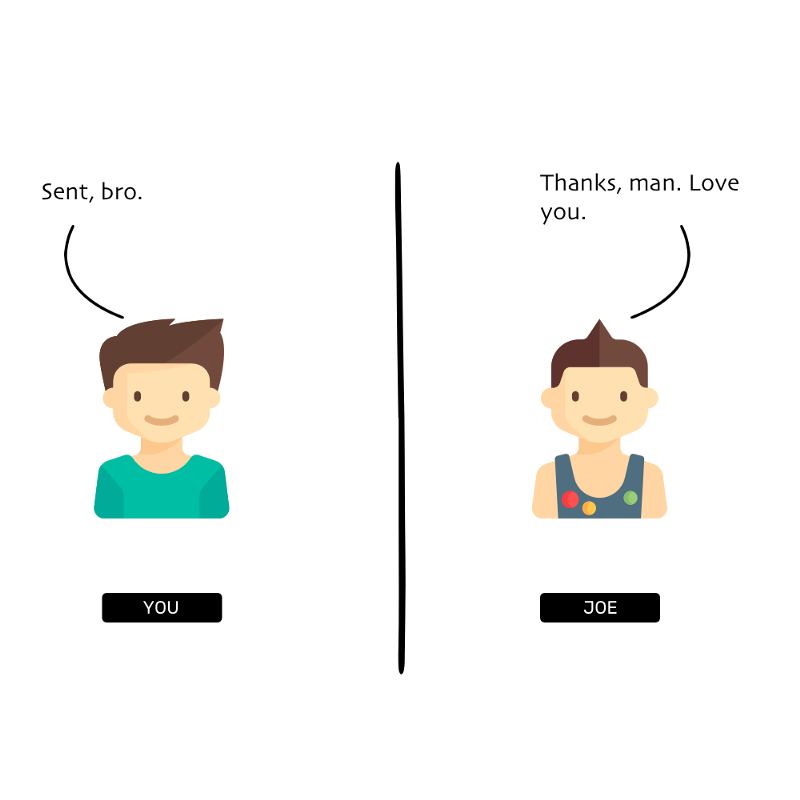
\includegraphics[width=80mm]{images/send_with_bank3.png}
    \end{figure}
  \end{frame}
  \begin{frame}{Motivation}
    \center Tillid mellem to parter afhænger af en \textcolor{RubineRed}{tredjepart}!
  \end{frame}
  \begin{frame}{Motivation}
      \center \textcolor{BrickRed}{Udfordring}:
      \center lav et system hvor vi kan overføre penge \\ uden at stole på banken
  \end{frame}
  \begin{frame}{Motivation}
      \center \textcolor{BrickRed}{Udfordring}:
      \center \sout{lav et system hvor vi kan overføre penge \\ uden at stole på banken}
      \center vedligehold en hovedbog uden hjælp fra en tredjepart
  \end{frame}
  \begin{frame}{Motivation}
      \center \textcolor{Dandelion}{Blockchain} to the rescue!
  \end{frame}
  \section{Mapper med papirer \ \ \ \ \ \ \ \ \ \ \ \ \ \ \ \ \ \ \ \ \ \ \ \ \ \ \ \ \ \ \ \ \ \ \ \ \ \ \small Jargon: Distributed ledger}

  \begin{frame}{Mapper med papirer}
    \begin{figure}[ht!]
    \centering
        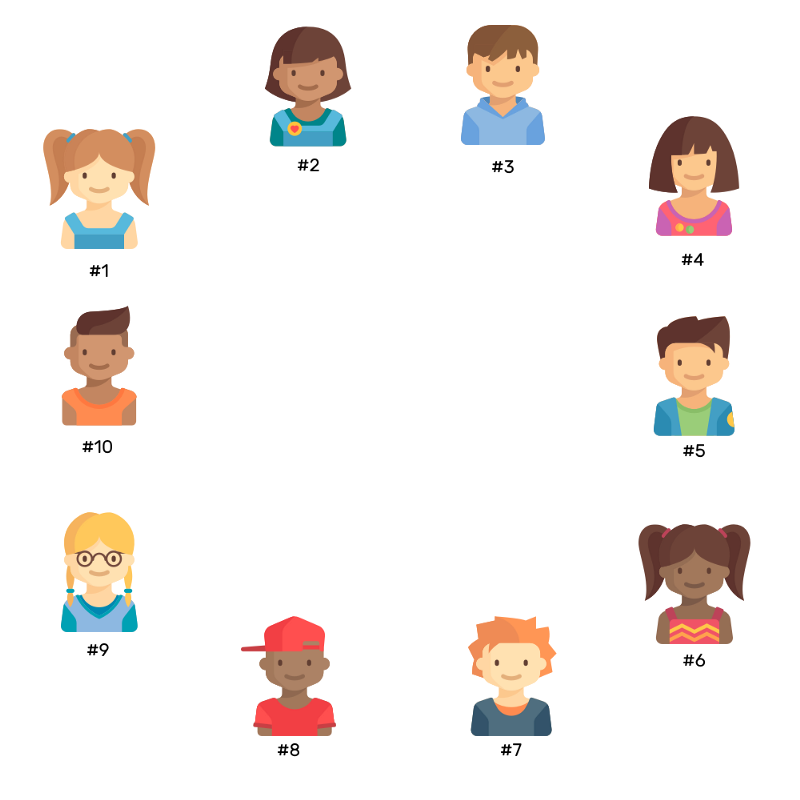
\includegraphics[width=80mm]{images/all_people.png}
    \end{figure}
  \end{frame}
  \begin{frame}{Mapper med papirer}
    \begin{figure}[ht!]
    \centering
    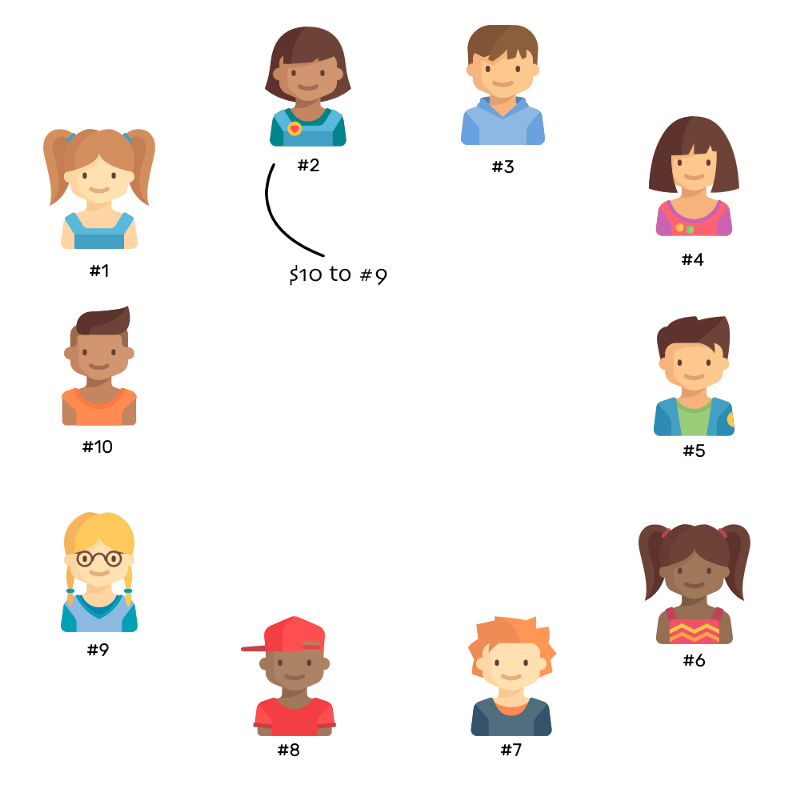
\includegraphics[width=80mm]{images/all_people_send.png}
    \end{figure}
  \end{frame}
  \begin{frame}{Mapper med papirer}
    \begin{figure}[ht!]
    \centering
    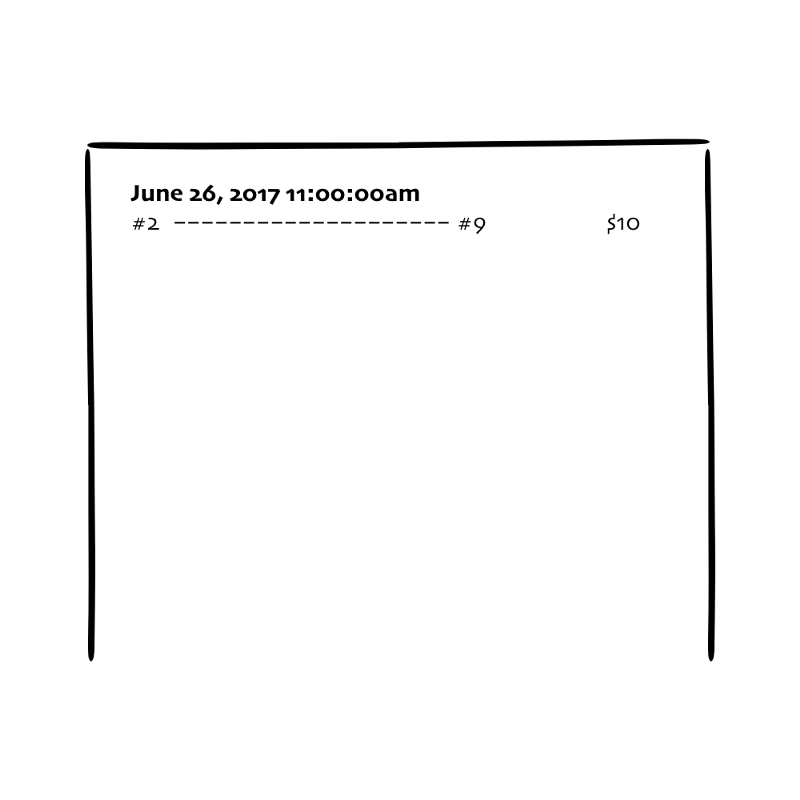
\includegraphics[width=80mm]{images/all_people_transaction.png}
    \end{figure}
  \end{frame}
  \begin{frame}{Mapper med papirer}
    \begin{figure}[ht!]
    \centering
    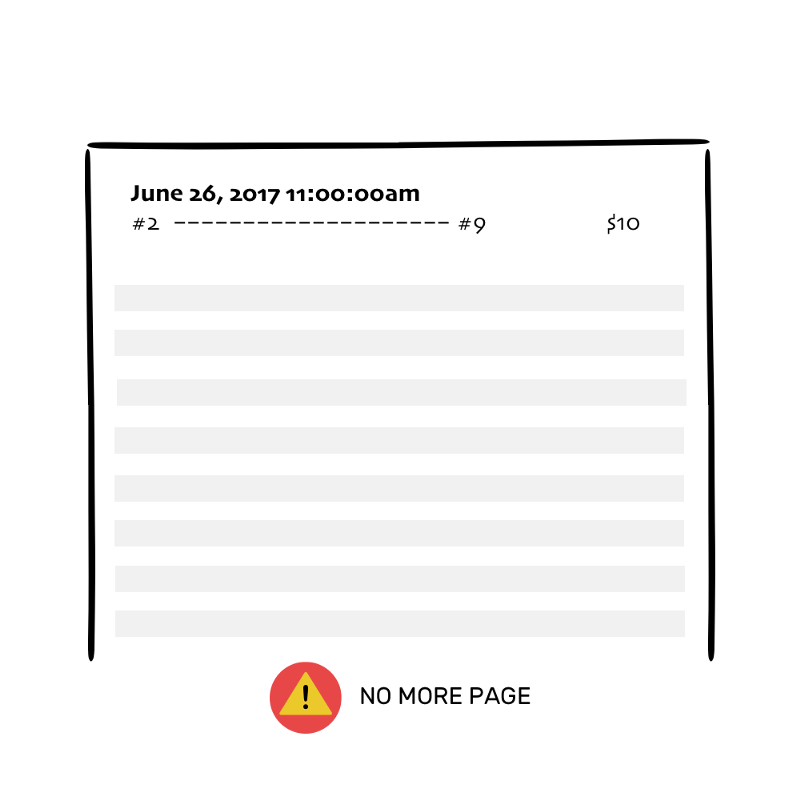
\includegraphics[width=80mm]{images/all_people_page_filled.png}
    \end{figure}
  \end{frame}
  \section{Magiske maskiner  \ \ \ \ \ \ \ \ \ \ \ \ \ \ \ \ \ \ \ \ \ \ \ \ \ \ \ \ \ \ \ \ \ \ \ \ \ \ \small Jargon: Cryptographic hash functions}
  \begin{frame}{Magiske maskiner}
    \begin{figure}[ht!]
    \centering
    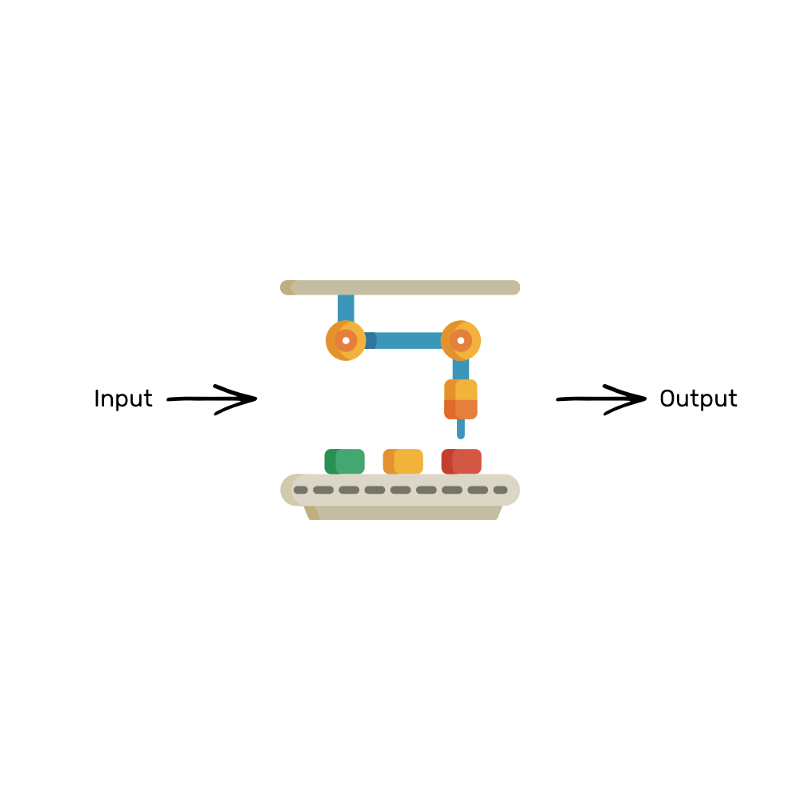
\includegraphics[width=80mm]{images/magic_machine.png}
    \end{figure}
  \end{frame}
  \begin{frame}{Magiske maskiner}
    \begin{figure}[ht!]
    \centering
    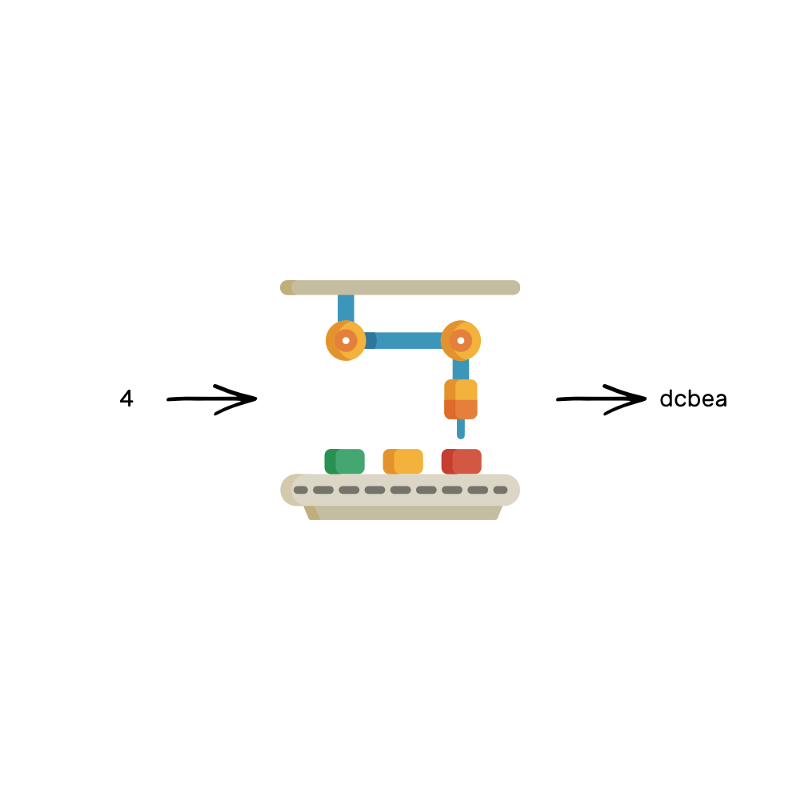
\includegraphics[width=80mm]{images/magic_machine_output1.png}
    \end{figure}
  \end{frame}
  \begin{frame}{Magiske maskiner}
    \begin{figure}[ht!]
    \centering
    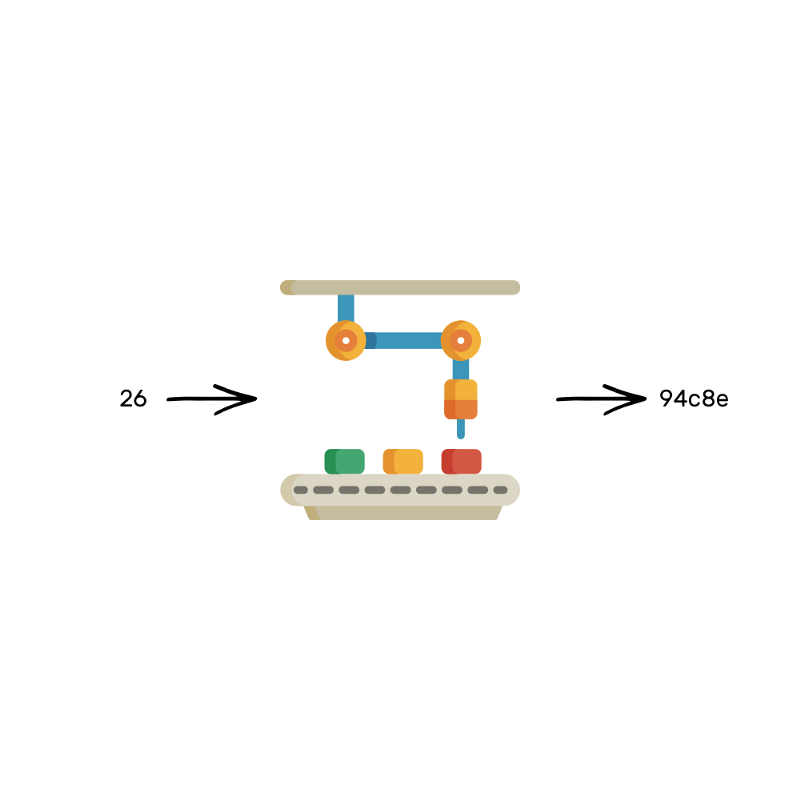
\includegraphics[width=80mm]{images/magic_machine_output2.png}
    \end{figure}
  \end{frame}
  \begin{frame}{Magiske maskiner}
    \begin{figure}[ht!]
    \centering
    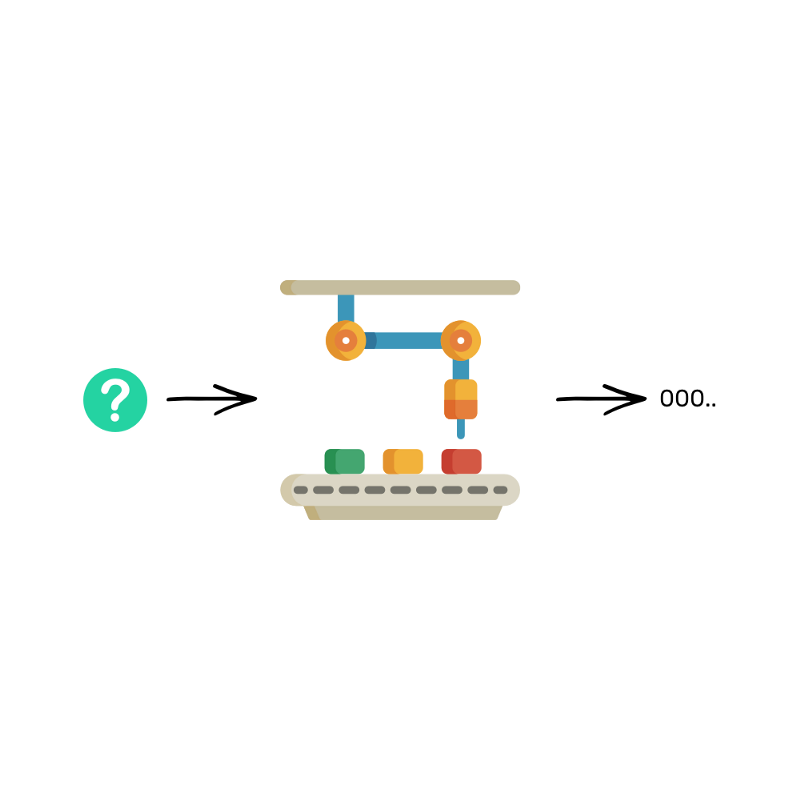
\includegraphics[width=80mm]{images/magic_machine_unknown_input.png}
    \end{figure}
  \end{frame}
  \begin{frame}{Magiske maskiner}
    \begin{figure}[ht!]
    \centering
    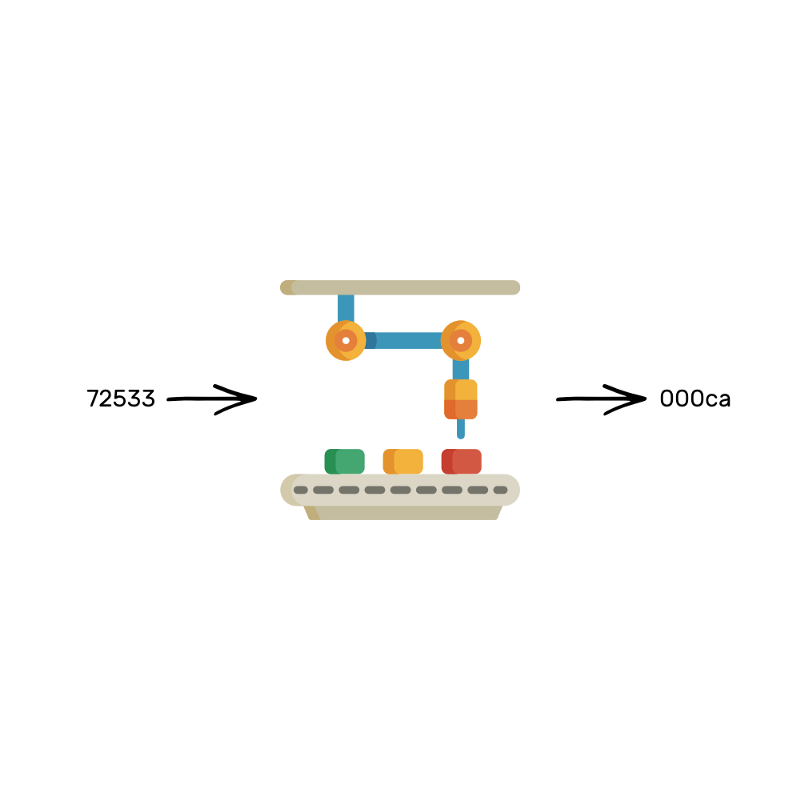
\includegraphics[width=80mm]{images/magic_machine_3zeros.png}
    \end{figure}
  \end{frame}
  \begin{frame}{Magiske maskiner}
    \begin{align*}
        \text{\textcolor{LimeGreen}{Input}} &\to \text{\textcolor{OrangeRed}{Output}}: nemt \\
        \text{\textcolor{OrangeRed}{Output}}&\to \text{\textcolor{LimeGreen}{Input}}: (ekstremt) \ svært
    \end{align*}
  \end{frame}
  \section{Forsegling  \ \ \ \ \ \ \ \ \ \ \ \ \ \ \ \ \ \ \ \ \ \ \ \ \ \ \ \ \ \ \ \ \ \ \ \ \ \ \small Jargon: Mining $\to$ Proof of work}
  \begin{frame}{Forsegling}
    \begin{figure}[ht!]
    \centering
    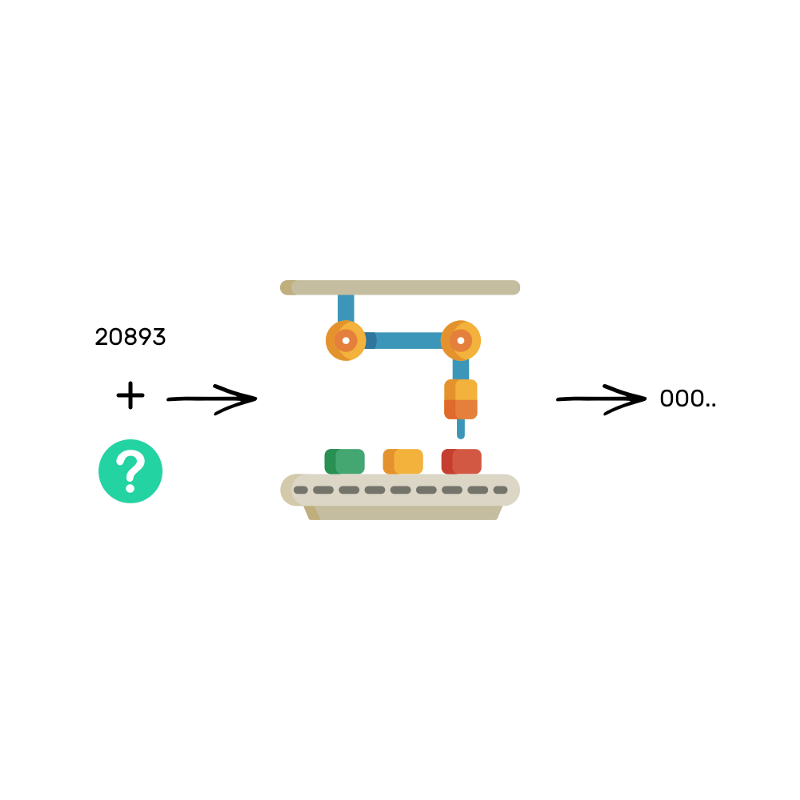
\includegraphics[width=80mm]{images/magic_machine_combination.png}
    \end{figure}
  \end{frame}
  \begin{frame}{Forsegling}
    \begin{figure}[ht!]
    \centering
    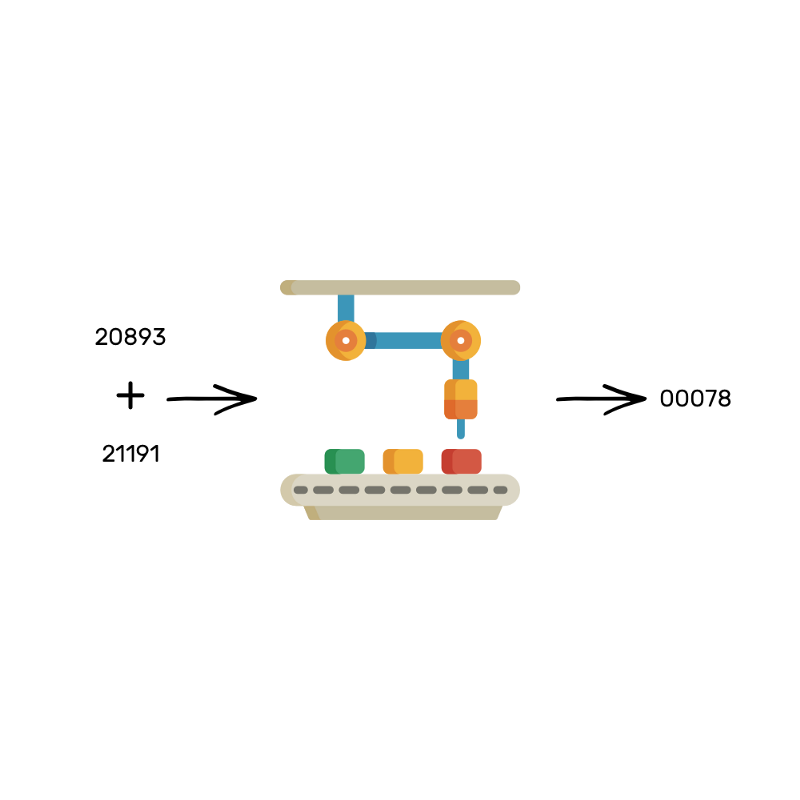
\includegraphics[width=80mm]{images/magic_machine_combination_found.png}
    \end{figure}
  \end{frame}
  \begin{frame}{Forsegling}
    \begin{figure}[ht!]
    \centering
    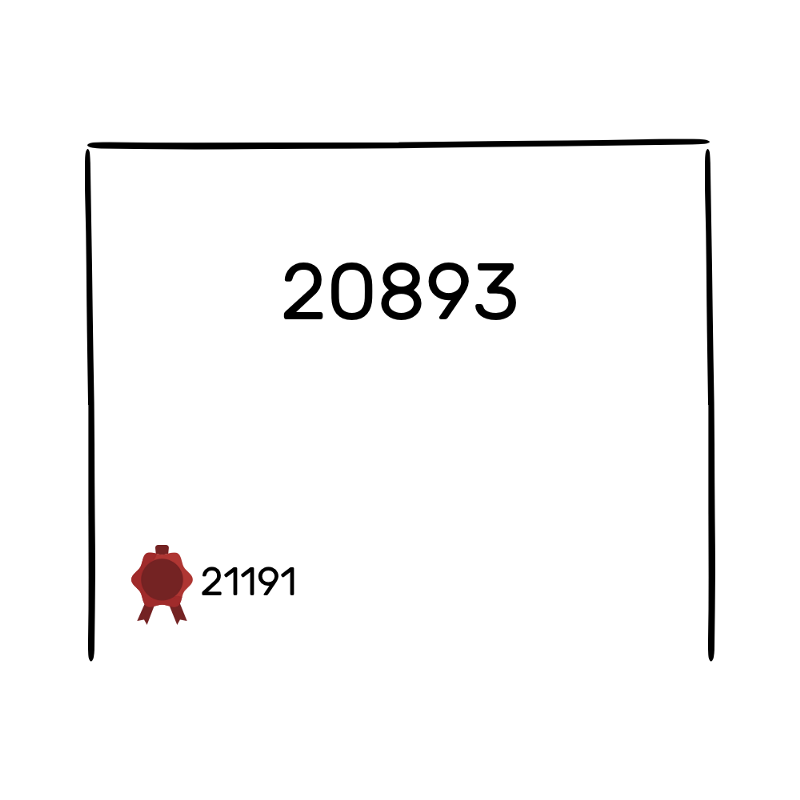
\includegraphics[width=80mm]{images/magic_machine_found.png}
    \end{figure}
  \end{frame}
  \begin{frame}{Forsegling}
    \begin{figure}[ht!]
    \centering
    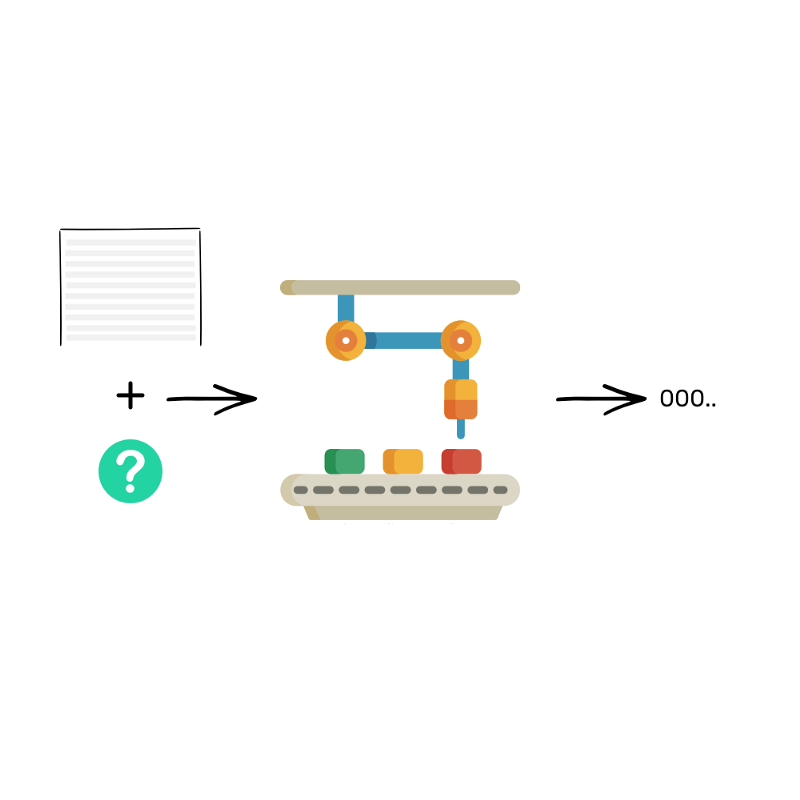
\includegraphics[width=80mm]{images/magic_machine_seal_page.png}
    \end{figure}
  \end{frame}
  \begin{frame}{Forsegling}
    \begin{figure}[ht!]
    \centering
    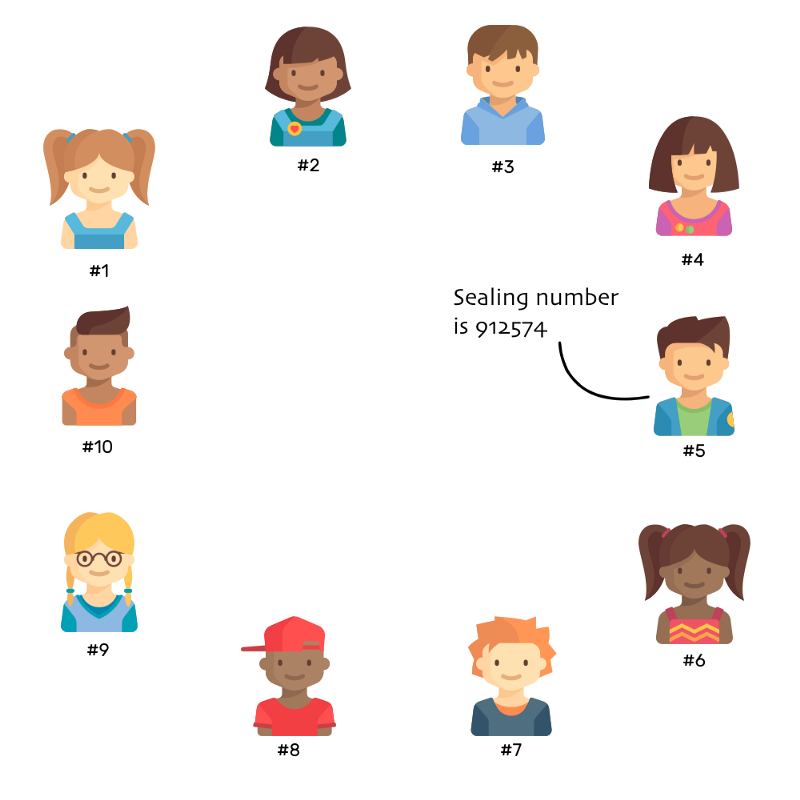
\includegraphics[width=80mm]{images/all_people_seal.png}
    \end{figure}
  \end{frame}
  \section{Hæfteklammer \ \ \ \ \ \ \ \ \ \ \ \ \ \ \ \ \ \ \ \ \ \ \ \ \ \ \ \ \ \ \ \ \ \ \ \ \ \ \small Jargon: 'chain' af Blockchain}
  \begin{frame}{Hæfteklammer}
    \begin{figure}[ht!]
    \centering
    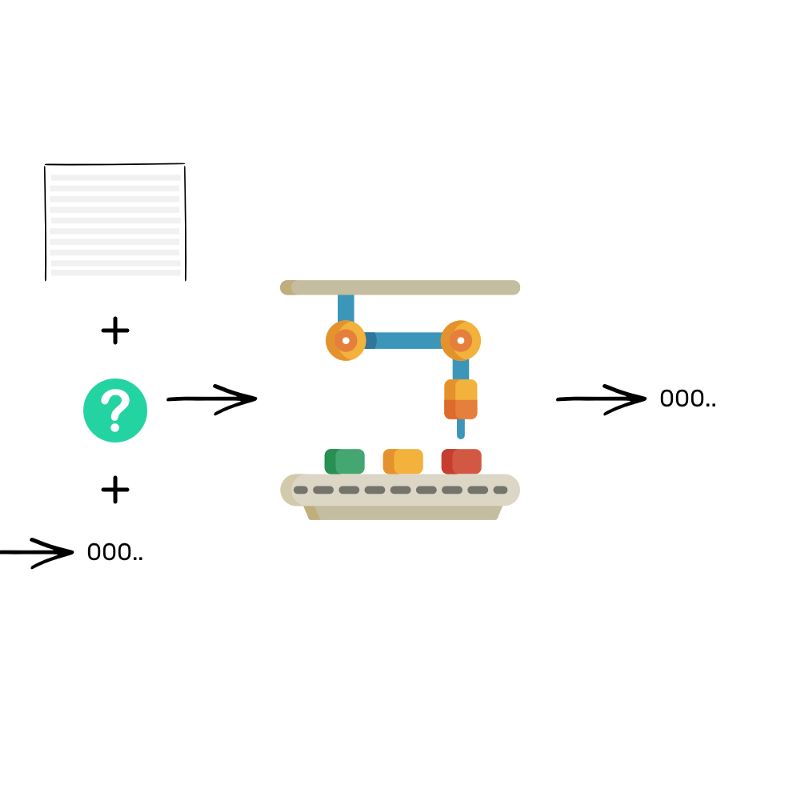
\includegraphics[width=80mm]{images/magic_machine_blockchain.png}
    \end{figure}
  \end{frame}
  \begin{frame}{Hæfteklammer}
    \begin{figure}[ht!]
    \centering
    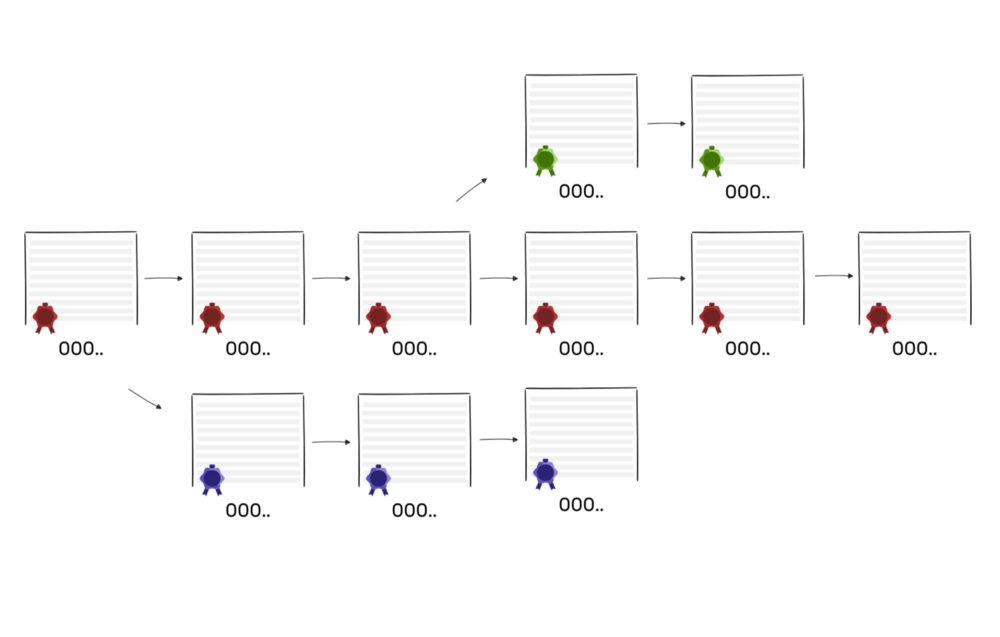
\includegraphics[width=80mm]{images/honest_chain.png}
    \end{figure}
  \end{frame}
\section{Underskrifter \ \ \ \ \ \ \ \ \ \ \ \ \ \ \ \ \ \ \ \ \ \ \ \ \ \ \ \ \ \ \ \ \ \ \ \ \ \ \small Jargon: Cryptograhpic Digital Signatures}
  \begin{frame}{Underskrifter}
    \begin{figure}[ht!]
    \centering
    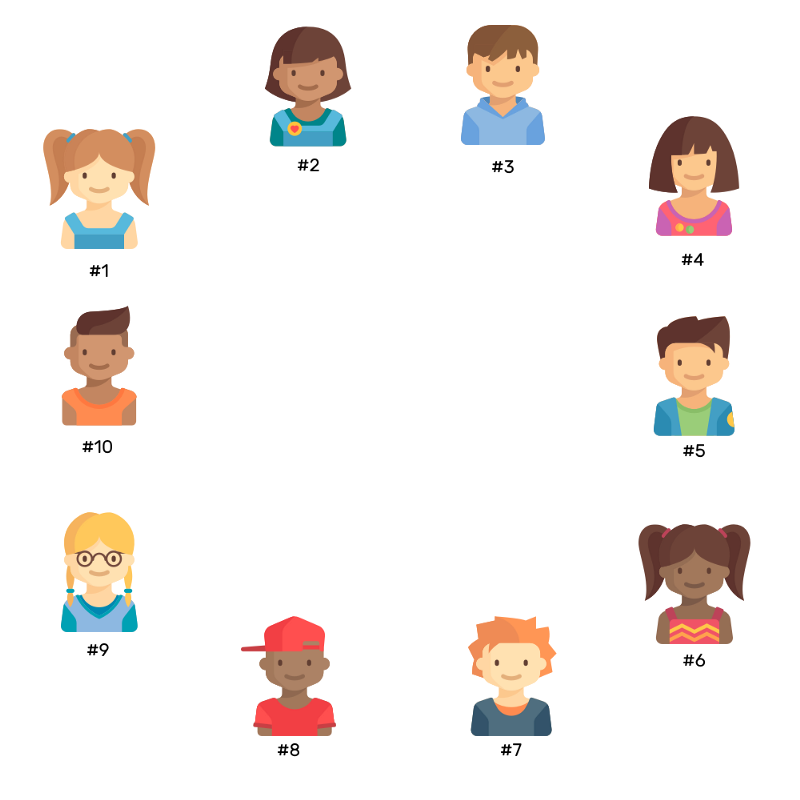
\includegraphics[width=80mm]{images/all_people.png}
    \end{figure}
  \end{frame}
  \begin{frame}{Underskrifter}
      \begin{align*}
      \textcolor{Orchid}{\#1} &\to \mathtt{1EJFbCLBiq9BNf5MZeXTGbPDdwnG2bDqtX}\\
          \textcolor{ProcessBlue}{\#2} &\to \mathtt{144burjrm7iqDt6q1LBpZ4oDwxd3Ln95yp}\\
          \textcolor{JungleGreen}{\#3} &\to \mathtt{1Kj5hMdZyEV46FDSfmqebvZemRqeJ6t2y5}\\
          \textcolor{BlueViolet}{\#4} &\to ...
      \end{align*}
  \end{frame}
  \begin{frame}{Underskrifter}
    \begin{figure}[ht!]
    \centering
    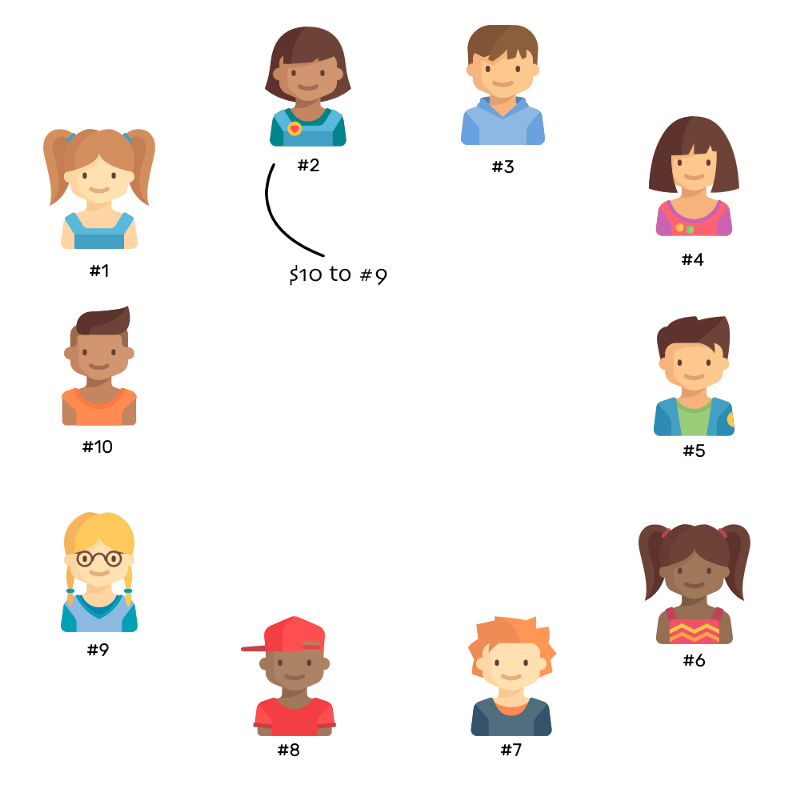
\includegraphics[width=80mm]{images/all_people_send.png}
    \end{figure}
  \end{frame}
  \begin{frame}{Underskrifter}
    \begin{figure}[ht!]
    \centering
    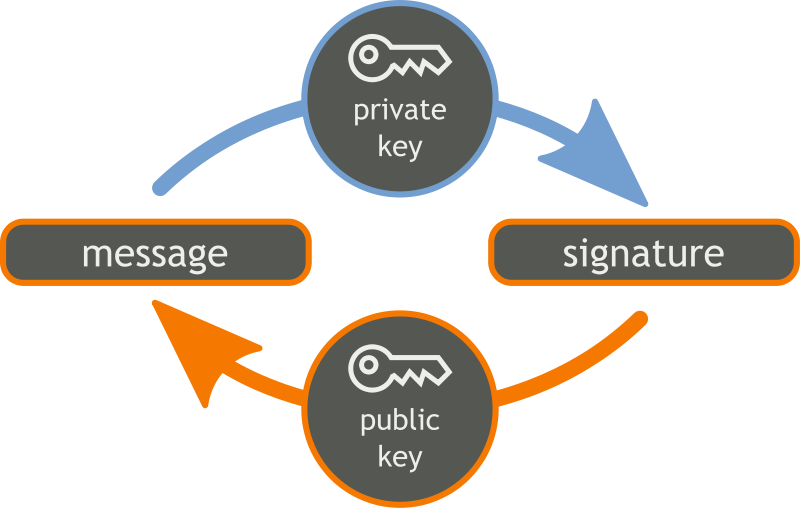
\includegraphics[width=80mm]{images/signature.png}
    \end{figure}
  \end{frame}
\section{Blockchain}
  \begin{frame}{Blockchain}
      \center \textcolor{Emerald}{Papirer} $+$ \textcolor{CarnationPink}{Mapper} $+$ \textcolor{Blue}{Segl} $+$ \textcolor{Green}{Hæfteklammer} $=$ \textcolor{Dandelion}{Blockchain}
  \end{frame}
  \begin{frame}{}
    \center \huge Tak for i aften! \\
  \end{frame}
\end{document}
